\documentclass[a4paper,11pt]{article}
\usepackage[osf]{mathpazo}
\usepackage{ms}
\usepackage[]{natbib}
\raggedright

\newcommand{\smurl}[1]{{\footnotesize\url{#1}}}



\usepackage{graphicx}

\title{Does population density moderate the importance of information in intraspecies contests?}
\author{
* John Wilshire$^1$, Will Cornwell$^1$ , Daniel Falster$^1$, Michael Kasumovic$^1$, \\
Daniel Noble$^1$}
\affiliation{
*final list and order undecided\\
$^1$ University of NSW\\
}
\date{}

\bibliographystyle{mee}

\usepackage[title,titletoc,toc]{appendix}

\mstype{Research Article}
\runninghead{A new framework for fighting}
\keywords{contests, density dependence}

\begin{document}
\mstitlepage
\noindent
% \doublespacing
% \linenumbers

\section{Summary}
% from old paper
The diversity of animal mating systems is astounding. In some of these
systems, very costly combat behaviour -- among males, among females, or
both -- is a feature of the mating process.  In other systems, resources
are divided among individuals in an entirely pacific process.  Can we
understand why? Animal combat strategies likely emerge from trade-offs
in investment in growth, mate seeking, and information gathering.
Willingness to engage in combat is a trait that evolves based on the
fitness landscape, which itself changes depending on both the
environment and the strategies of other individuals.  Using recently
developed methods for modelling dynamic fitness landscapes, we examine:
(1) why combat behaviours arise, (2) under what conditions combat
behaviours are evolutionarily stable, and (3) when different combat
strategies co-exist.  We hypothesize that the reliability and
"public-ness" of information is an important feature driving combat or
lack thereof in many animal systems.

\section{Introduction}
Evolution of animal personalities: \citep{Wolf-2007,Wolf-2012} show can have
coexistence of risky, explorative strategies and risk-averse strategies.

Animal personalities linked to other life history traits: \citep{Biro-2008}

Individual-based models of natural selection: \citep{MGonigle-2012}



\section{Methods}
\begin{figure}
  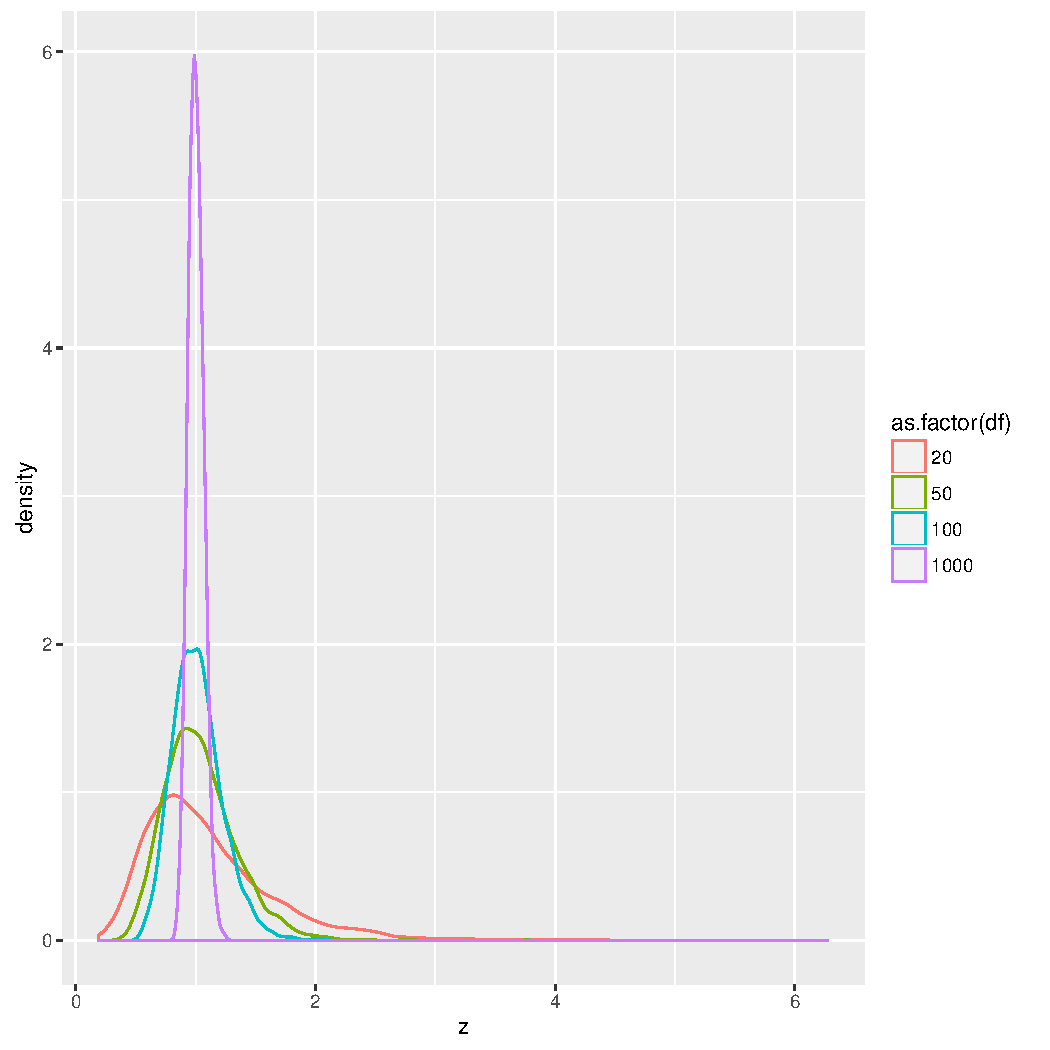
\includegraphics[width=\textwidth]{figures/fight_randomness.pdf}
  \caption{Randomness in perception of self and opponent}
\end{figure}

\section{Results}

\begin{figure}
  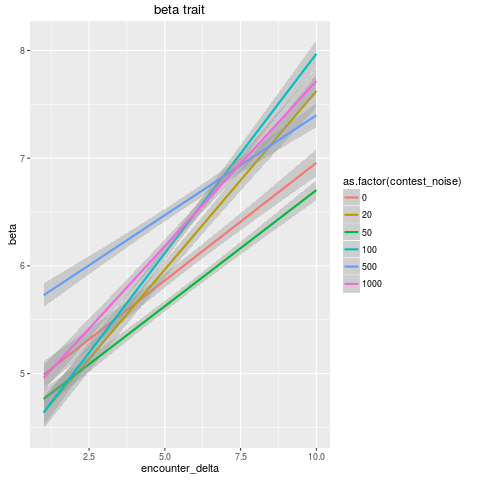
\includegraphics[width=\textwidth]{figures/beta_plot.png}
  \caption{$\beta$ trait with increasing average time between encounters. coloured by level of
  reliabilty of in self and opponent mass judgements. }
\end{figure}

\begin{figure}
  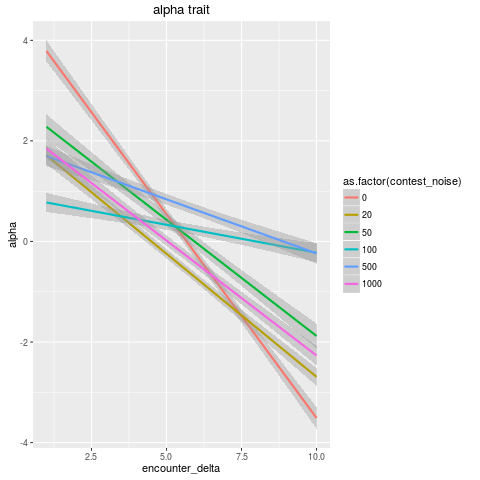
\includegraphics[width=\textwidth]{figures/alpha_plot.png}
  \caption{Randomness in perception of self and opponent}
\end{figure}


\section{Discussion}

\begin{center} % this file is cfeated by remake 
    % latex table generated in R 3.3.2 by xtable 1.8-2 package
% Sun Feb 12 14:19:55 2017
\begin{table}[ht]
\centering
\begin{tabular}{rlr}
  \hline
 & Parameter & . \\ 
  \hline
1 & max\_gens & 10000.00 \\ 
  2 & males\_per\_winner & 10.00 \\ 
  3 & num\_nests & 100.00 \\ 
  4 & encounter\_delta & 1.00 \\ 
  5 & metabolism & 1.00 \\ 
  6 & female\_mat\_time & 10.00 \\ 
  7 & maturation\_rate & 1.00 \\ 
  8 & mutation\_rate & 0.00 \\ 
  9 & mutation\_sd & 0.01 \\ 
  10 & mass\_to\_energy & 10.00 \\ 
  11 & growth\_a & 0.50 \\ 
  12 & growth\_b & 0.10 \\ 
  13 & initial\_mass & 5.00 \\ 
  14 & alpha\_mean & 0.00 \\ 
  15 & alpha\_sd & 3.00 \\ 
  16 & beta\_sd & 3.00 \\ 
  17 & beta\_max & 10.00 \\ 
  18 & beta\_mean & 0.00 \\ 
  19 & verbose & 0.00 \\ 
  20 & log\_every & 1000.00 \\ 
  21 & contest\_noise & 0.00 \\ 
  22 & quiet & 1.00 \\ 
   \hline
\end{tabular}
\caption{The Parameters used to run the model} 
\end{table}

\end{center}
\clearpage
\bibliography{refs}

\end{document}
